
\providecommand{\sSet}{s\mathcal{S}et}
\providecommand{\colim}{\operatorname{colim}}

\section{锥形极限与余极限}\label{sec:conical-limits-and-colimits}

试考虑一支图表 $F\colon\mathcal{J}\to\mathcal{C}$，其由一个 1-\trCategory{}
$\mathcal{J}$ 标引，而取值于一个 $\mathcal{V}$-\trCategory{} $\mathcal{C}$。
图表 $F$ 之上带峰顶 $\ell\in\mathcal{C}$ 的一支\trCone{} $\lambda$ 是一支极限
锥，若与 $\lambda$ 的复合诱导诸 hom-集之间的一个双射
\[ \mathcal{C}(x,\ell)_{0}\xrightarrow[\ \simeq\ ]{\ \lambda\circ-\ }
   \lim_{j\in\mathcal{J}}\mathcal{C}(x,Fj)_{0} \]
对一切 $x\in\mathcal{C}$。若 $\mathcal{V}$ 容许形状为 $\mathcal{J}$ 的%
\trLimit，则该复合映射提升入 $\mathcal{V}$ 中，并且，断言极限锥之通常%
\trUniversalProperty{}的一个更强版本乃是自然之事：要求与 $\lambda$ 的复合诱导
诸 $\mathcal{V}$-对象之间的一个\trIsomorphism，而不只是诸 hom-集之间的一个。
这就给出了取值于一个\trEnrichedCategory{}的图表之\emph{锥形极限}的概念。%
\emph{锥形余极限}对偶地定义（见\cref{def:conical-limit-colimit}）。

底集函子 $(-)_{0}\coloneqq\mathcal{V}(1,-)\colon\mathcal{V}\to\mathcal{S}et$
保持\trLimit，并把 $\mathcal{V}$ 中的\trIsomorphism{}带为诸集合之间的双射。
于是，锥形极限必然定义 1-范畴的\trLimit，故我们特别关注：要把一个 1-范畴的%
\trLimit{}富集成一个锥形极限，究竟需要些什么。沿这条路线的第一个观察是：取值
于\trCartesianClosed{}\trCategory{} $\mathcal{V}$ 的图表之\trLimit{}与%
\trColimit{}总是富集而定义锥形极限与锥形余极限。

\begin{lemma}\label{lem:cc-conical}
若 $\mathcal{V}$ 是一个\trCartesianClosed{}\trCategory，则图表
$F\colon\mathcal{J}\to\mathcal{V}$ 之上的任一 1-范畴的极限锥
$\lambda\colon\Delta\lim F\Rightarrow F$，或其之下的任一 1-范畴的余极限锥
$\gamma\colon F\Rightarrow\Delta\colim F$，都产生诸\trIsomorphism
\[ (\lim F)^{v}\cong\lim_{j\in\mathcal{J}}(Fj)^{v}
   \qquad\text{以及}\qquad
   v^{\colim F}\cong\lim_{j\in\mathcal{J}^{\mathrm{op}}}v^{Fj} \]
其居于 $\mathcal{V}$ 之中，且在 $v\in\mathcal{V}$ 中是 $\mathcal{V}$-自然的。
\end{lemma}

\begin{proof}
对任何 $v\in\mathcal{V}$，指数\trFunctor{}
$(-)^{v}\colon\mathcal{V}\to\mathcal{V}$ 是乘积\trFunctor{}
$-\times v\colon\mathcal{V}\to\mathcal{V}$ 的\trRightAdjoint；正因如此，它保持%
\trLimit，这就产生了陈述中的第一个\trIsomorphism；而
$v^{-}\colon\mathcal{V}^{\mathrm{op}}\to\mathcal{V}$ 作为互为右伴随者，则把%
\trColimit{}带为\trLimit，这就建立了第二个。
\end{proof}

从本节余下部分起，设 $\mathcal{V}$ 是一个\trComplete{}\trCartesianClosed{}%
\trCategory，从而编码锥形极限与锥形余极限之\trUniversalProperty{}的那些
$\mathcal{V}$ 中的\trLimit{}被设定为存在。

\begin{definition}\label{def:conical-limit-colimit}
设 $\mathcal{C}$ 是一个 $\mathcal{V}$-\trCategory{}并设 $\mathcal{J}$ 是一个
小 1-\trCategory。非富集图表 $F\colon\mathcal{J}\to\mathcal{C}$ 的%
\textbf{锥形极限}（conical limit）由一个对象 $\ell\in\mathcal{C}$ 与一支%
\trCone{} $\lambda\colon\Delta\ell\Rightarrow F$ 给出，后者诱导诸 hom-对象
之间的一个 $\mathcal{V}$-自然\footnote{对任何\trCone{}
$\lambda\colon\Delta\ell\Rightarrow F$——不必是极限锥——复合定义一个映射
$\lambda\circ-\colon\mathcal{C}(x,\ell)\to\lim\limits_{j\in\mathcal{J}}\mathcal{C}(x,Fj)$，
其在 $x$ 中是 $\mathcal{V}$-自然的（见\cref{ex:conical-map-vnatural}）。其证
由与\cref{exa:post-composition-vnatural-transformation}中所用者本质相同的论证
给出——该论证证明：富集范畴之底范畴中的诸箭头在诸可表示函子之间诱导富集%
\trNaturalTransformation。于是，刻画锥形极限的那个\trUniversalProperty{}之
内容即在于：这个 $\mathcal{V}$-自然映射是\trInvertible。}\trIsomorphism
\[ \mathcal{C}(x,\ell)\xrightarrow[\ \simeq\ ]{\ \lambda\circ-\ }
   \lim_{j\in\mathcal{J}}\mathcal{C}(x,Fj)
   \qquad\in\ \mathcal{V} \]
对一切 $x\in\mathcal{C}$。对偶地，\textbf{锥形余极限}（conical colimit）由一
个对象 $c\in\mathcal{C}$ 与一支\trCone{} $\gamma\colon F\Rightarrow\Delta c$
给出，后者诱导一个 $\mathcal{V}$-自然\trIsomorphism
\[ \mathcal{C}(c,x)\xrightarrow[\ \simeq\ ]{\ \gamma^{*}\ }
   \lim_{j\in\mathcal{J}^{\mathrm{op}}}\mathcal{C}(Fj,x)
   \qquad\in\ \mathcal{V} \]
对一切 $x\in\mathcal{C}$。
\end{definition}

刻画锥形极限与锥形余极限的那些\trIsomorphism，与刻画 1-范畴的\trLimit{}和%
\trColimit{}的那些通常\trIsomorphism{}极为相似，只是有一个非常重要的差别：它
们设定的是 $\mathcal{V}$ 中的\trIsomorphism，而非 $\mathcal{S}et$ 中的%
\trIsomorphism。在 $\mathcal{V}=\sSet$ 的情形，这个单纯集之间的%
\trIsomorphism{}所底下的那个顶点之间的\trIsomorphism{}描述的正是通常的
1-范畴\trUniversalProperty。称一个\trLimit{}是\emph{锥形的}而不只是%
\emph{1-范畴的}，即是断言这个\trUniversalProperty{}延伸到一切正维数。

检视\cref{def:conical-limit-colimit}，我们立即看到：

\begin{proposition}\label{prop:conical-representables}
一支 1-范畴的极限锥是锥形的，恰当时它被一切取值于 $\mathcal{V}$ 中的可表示
函子 $\mathcal{C}(x,-)\colon\mathcal{C}\to\mathcal{V}$ 所保持；而一支 1-范畴
的余极限锥是锥形的，恰当时它被一切取值于 $\mathcal{V}$ 中的可表示函子
$\mathcal{C}(-,x)\colon\mathcal{C}^{\mathrm{op}}\to\mathcal{V}$ 所保持。
\end{proposition}

\cref{lem:cc-conical}之证明可加以推广以证：

\begin{proposition}\label{prop:tensors-cotensors-conical}
在一个张量化的富集范畴 $\mathcal{C}$ 中，一切 1-范畴的\trLimit{}都是锥形的；
而在一个余张量化的富集范畴 $\mathcal{C}$ 中，一切 1-范畴的\trColimit{}都是
锥形的。
\end{proposition}

\begin{proof}
由\cref{prop:conical-representables}，为证 $\mathcal{V}$-\trCategory{}
$\mathcal{C}$ 中的一个 1-范畴的\trLimit{}是锥形的，只需证明它被诸取值于
$\mathcal{V}$ 中的可表示函子 $\mathcal{C}(x,-)\colon\mathcal{C}\to\mathcal{V}$
对一切 $x\in\mathcal{C}$ 所保持。若 $\mathcal{C}$ 容许张量，则这些\trFunctor{}%
中的每一个都容有一个\trLeftAdjoint；作为\trRightAdjoint，后者必然保持陈述中
的那些 1-范畴的\trLimit。
\end{proof}

与\cref{prop:conical-representables}相类比，我们有：

\begin{proposition}\label{prop:cotensor-preservation}
设 $\mathcal{C}$ 在 $\mathcal{V}$ 上富集且余张量化。非富集图表
$F\colon\mathcal{J}\to\mathcal{C}$ 的一个\trLimit{}是一个锥形极限，当且仅当
它被与一切对象 $v\in\mathcal{V}$ 的余张量所保持。
\end{proposition}

\begin{proof}
余张量是 $\mathcal{V}$-富集的\trRightAdjoint，后者保持锥形极限。其实质在于：
被余张量保持即足以把一个 1-范畴的\trLimit{}富集为一个 $\mathcal{V}$-范畴的%
\trLimit。

由\cref{prop:conical-representables}，一支 1-范畴的极限锥
$\lambda\colon\Delta\ell\Rightarrow F$ 是锥形的，恰当时它被一切取值于
$\mathcal{V}$ 中的可表示函子 $\mathcal{C}(x,-)\colon\mathcal{C}\to\mathcal{V}$
所保持。为见自然映射
\[ \mathcal{C}(x,\ell)\xrightarrow{\ \lambda\circ-\ }
   \lim_{j\in\mathcal{J}}\mathcal{C}(x,Fj) \]
是 $\mathcal{V}$ 中的一个\trIsomorphism，我们诉诸非富集的\trYonedaLemma{}并
论证：对任何 $v\in\mathcal{V}$，在施加非富集可表示函子
$\mathcal{V}(v,-)\colon\mathcal{V}\to\mathcal{S}et$ 时，这个映射诱导一个%
\trIsomorphism。为见这一可逆性，注意到诱导出的 hom-集之间的映射恰好居于如下
交换图表之中
\begin{center}
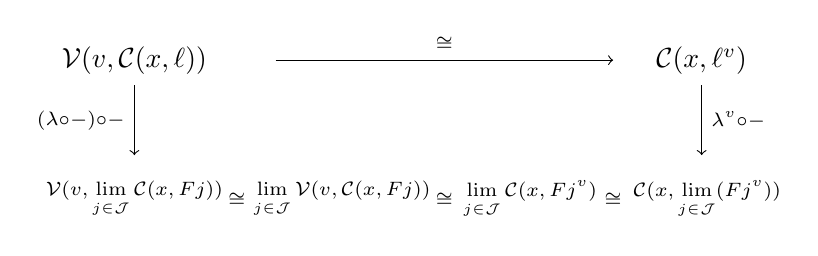
\begin{tikzpicture}[x=1em,y=1.4em]
  \node (tl) at (0,2.2) {$\mathcal{V}(v,\mathcal{C}(x,\ell))$};
  \node (tr) at (20.5,2.2) {$\mathcal{C}(x,\ell^{v})$};
  \draw[->] (5.1,2.2) -- node[above]{$\scriptstyle\cong$} (17.3,2.2);
  \draw[->] (0,1.55) -- node[left]{$\scriptstyle(\lambda\circ-)\circ-$} (0,-0.25);
  \draw[->] (20.5,1.55) -- node[right]{$\scriptstyle\lambda^{v}\circ-$} (20.5,-0.25);
  \node[font=\scriptsize] (b1) at (0,-1.4)
    {$\mathcal{V}(v,\displaystyle\lim_{j\in\mathcal{J}}\mathcal{C}(x,Fj))$};
  \node[font=\scriptsize] at (3.7,-1.4) {$\cong$};
  \node[font=\scriptsize] (b2) at (7.5,-1.4)
    {$\displaystyle\lim_{j\in\mathcal{J}}\mathcal{V}(v,\mathcal{C}(x,Fj))$};
  \node[font=\scriptsize] at (11.2,-1.4) {$\cong$};
  \node[font=\scriptsize] (b3) at (14.3,-1.4)
    {$\displaystyle\lim_{j\in\mathcal{J}}\mathcal{C}(x,Fj^{v})$};
  \node[font=\scriptsize] at (17.3,-1.4) {$\cong$};
  \node[font=\scriptsize] (b4) at (20.7,-1.4)
    {$\mathcal{C}(x,\displaystyle\lim_{j\in\mathcal{J}}(Fj^{v}))$};
\end{tikzpicture}
\end{center}
其中诸水平\trIsomorphism{}表达余张量的非富集\trUniversalProperty，以及非富集
可表示函子保持\trLimit{}这一事实。

说诸余张量保持\trLimit{} $\ell\cong\lim\limits_{j\in\mathcal{J}}Fj$，即意指
$\ell^{v}\cong(\lim\limits_{j\in\mathcal{J}}Fj)^{v}\cong\lim\limits_{j\in\mathcal{J}}(Fj)^{v}$；
故由\trYonedaLemma，右竖直的映射是一个\trIsomorphism，从而左竖直的映射亦然。
\end{proof}

\subsection*{练习}

\begin{exercise}\label{ex:conical-map-vnatural}
试考虑一支图表 $F\colon\mathcal{J}\to\mathcal{C}$——其由一个 1-\trCategory{}%
标引而取值于一个 $\mathcal{V}$-\trCategory——以及一支\trCone{}
$\lambda\colon\Delta\ell\Rightarrow F$。假设 $\mathcal{V}$ 容有形状为
$\mathcal{J}$ 的\trLimit，试定义一个典范映射
$\lambda\circ-\colon\mathcal{C}(x,\ell)\to\lim\limits_{j\in\mathcal{J}}\mathcal{C}(x,Fj)$，
并沿\cref{exa:post-composition-vnatural-transformation}的路线论证：它是
$\mathcal{V}$-自然的。
\end{exercise}

\begin{exercise}[{\cite[第~306~页]{bib67}}]\label{ex:2cat-tensors-conical}
将\cref{prop:tensors-cotensors-conical}之结果特殊化，以证明下述结论：在任何
一个容许与\trWalkingArrow{}范畴 $2$ 取张量的 2-\trCategory{} $\mathcal{C}$
中，$\mathcal{C}$ 所容有的任何 1-范畴的\trLimit{}都自动是锥形的。%
\footnote{本陈述断言：与 $2$ 取张量之存在，蕴涵 1 维\trLimit{}的%
\trUniversalProperty{}自动带有一个额外的 2 维面向，如围绕第 1 章中的%
\cref{prop:cartesian-closure}的讨论所例示的那样。}
\end{exercise}

